%%%%%%%%%%%%%%%%%%%%%%%%%%%%%%%%%%%%%%%%%%%%%%%%%%%%%%%%%%%%%%%
%
% Welcome to Overleaf --- just edit your LaTeX on the left,
% and we'll compile it for you on the right. If you open the
% 'Share' menu, you can invite other users to edit at the same
% time. See www.overleaf.com/learn for more info. Enjoy!
%
%%%%%%%%%%%%%%%%%%%%%%%%%%%%%%%%%%%%%%%%%%%%%%%%%%%%%%%%%%%%%%%

\documentclass{beamer}
\usetheme{Copenhagen}
\setbeamertemplate{navigation symbols}{}
\usepackage[utf8]{inputenc}
\usepackage{listings}
\usepackage{graphicx}
\usepackage[export]{adjustbox}
\graphicspath{ {./photos/} }

\title{Linux Empowered Automation for Developers}
\author{Gabriel Hanu}
\institute{UBB - Mathematics and Computer Science}
\date{2024}

\begin{document}

\frame{\titlepage}

% 1 SLIDE
\begin{frame}

\frametitle{Why do I like Linux? }

    \begin{figure}

        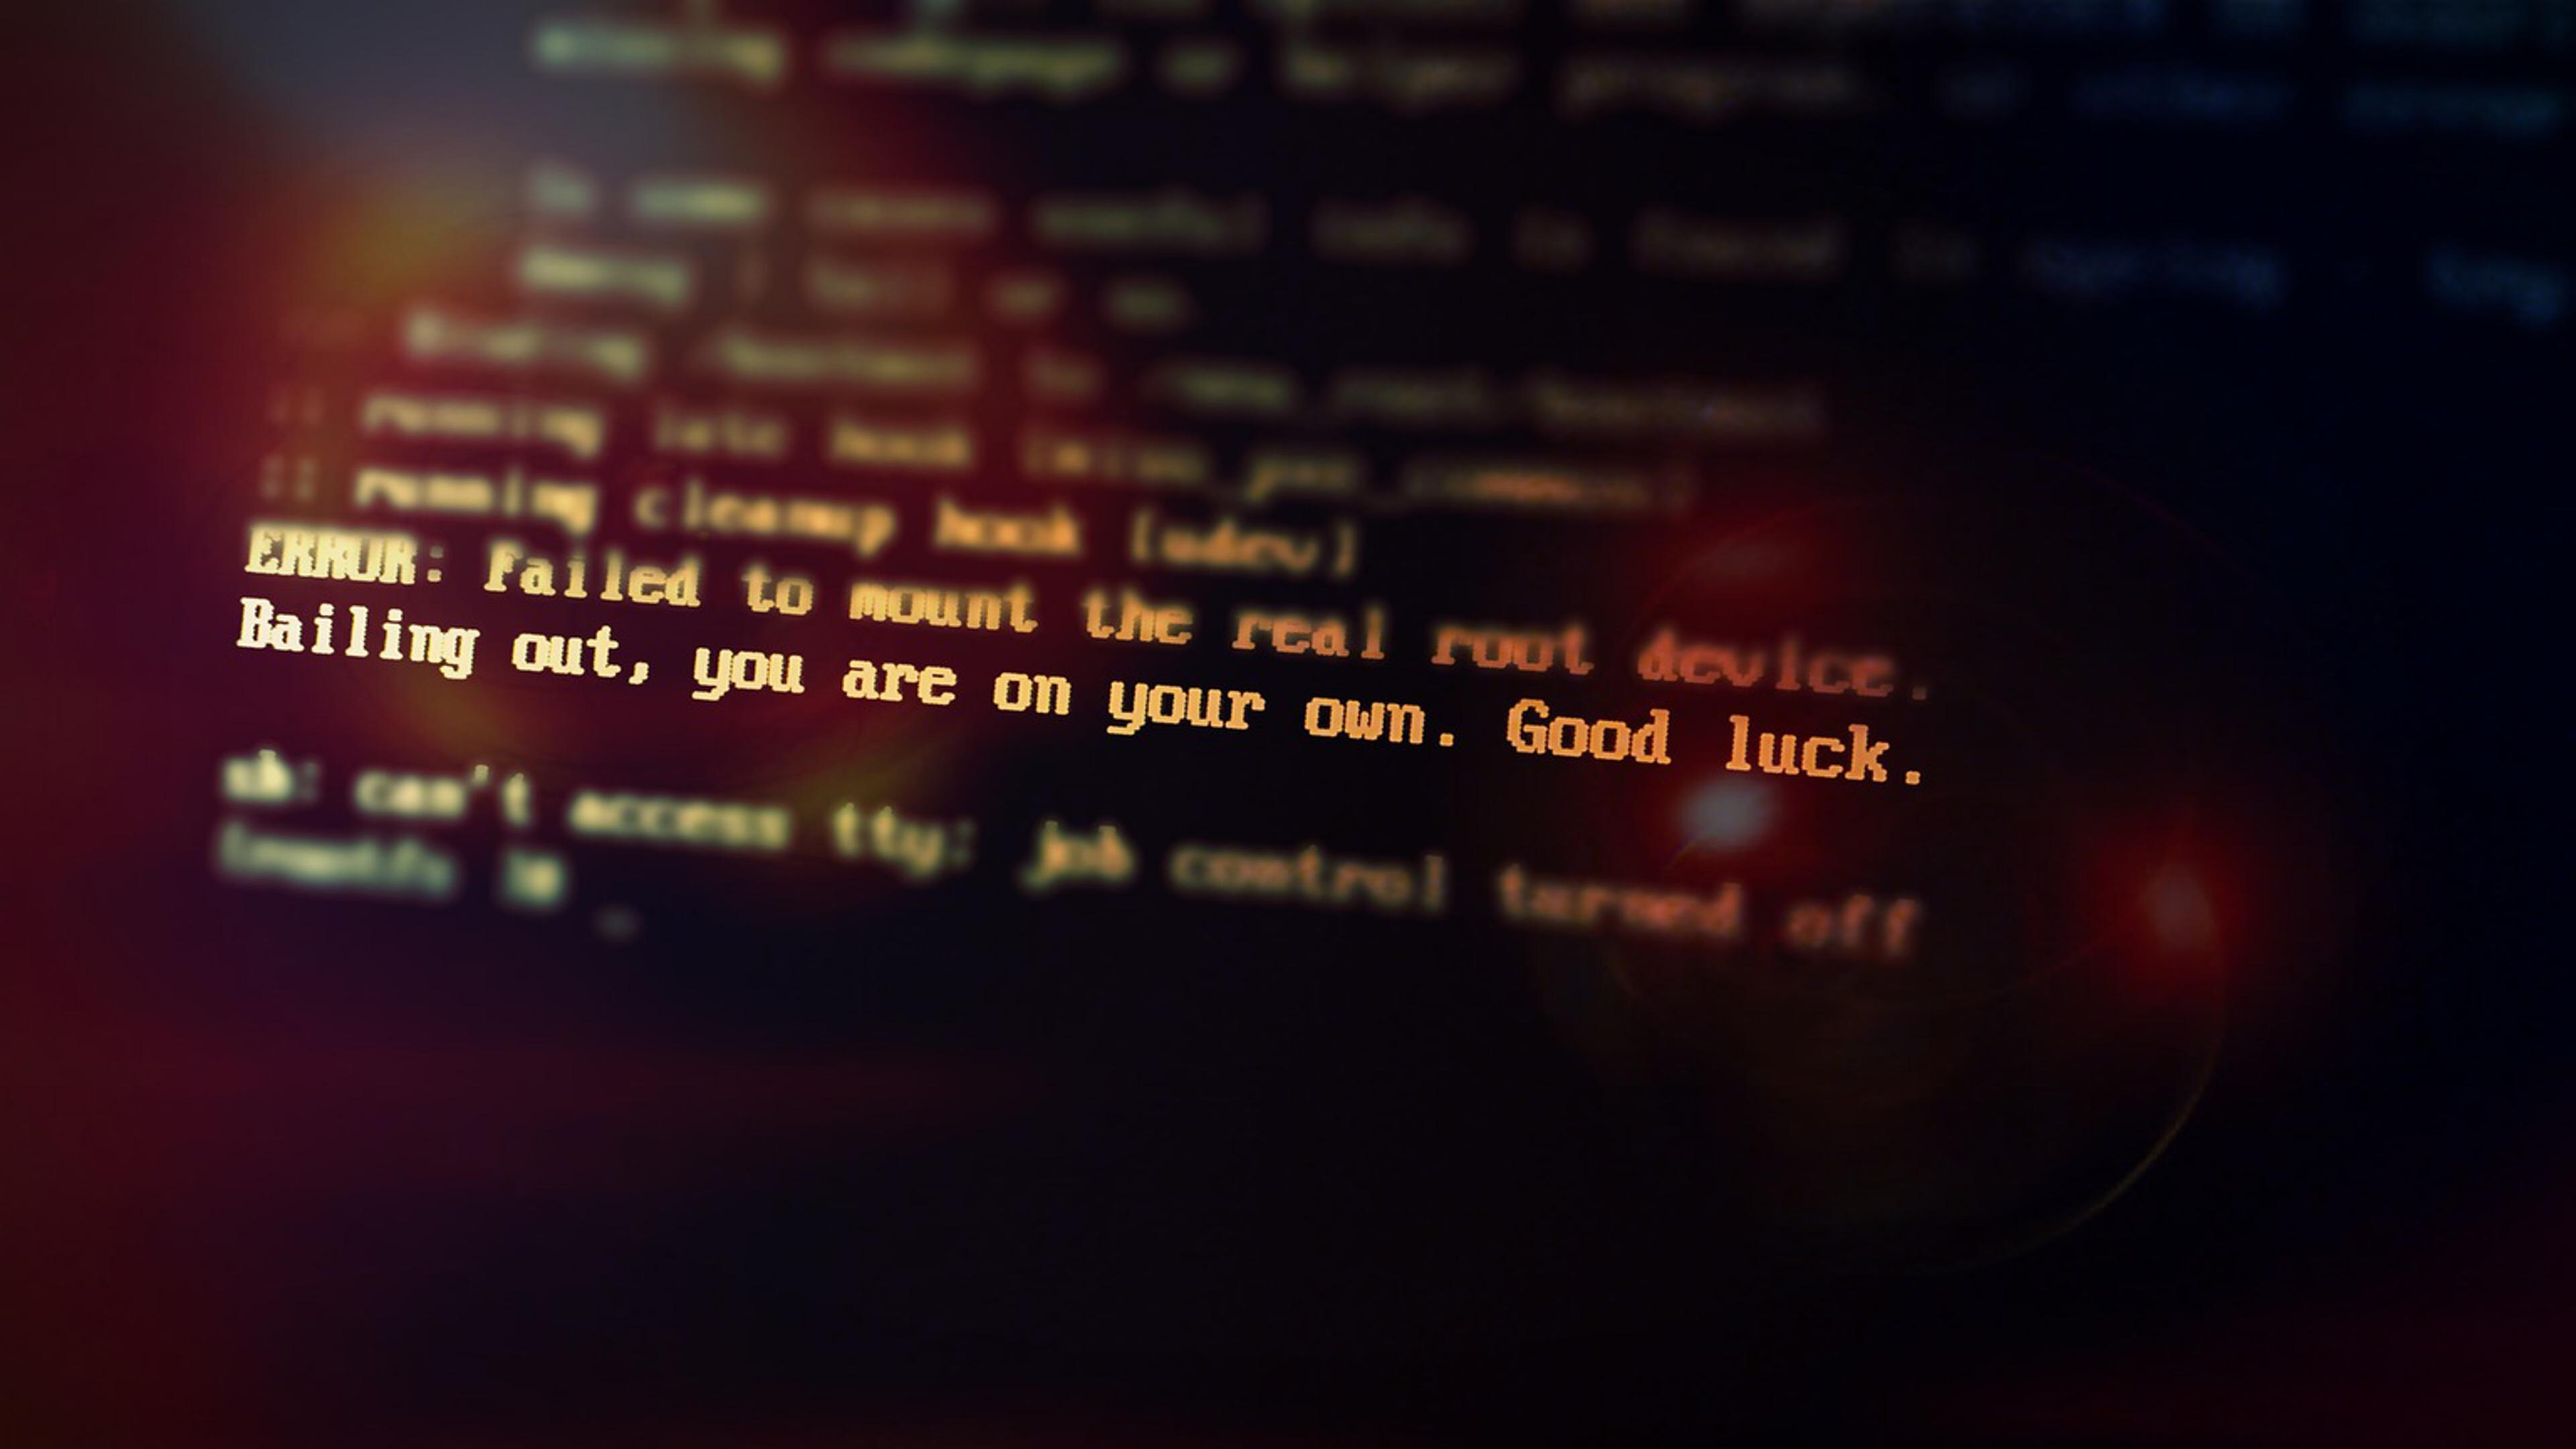
\includegraphics[width=0.8\linewidth]{whyilikelinux}

        \label{fig:whyilikelinux}

    \end{figure}
    \centering \small This may require a bit of a story...
\end{frame}

% 2 SLIDE
\begin{frame}

\frametitle{Useful resources}
\begin{itemize}
    \item Linux Bible
    \item Manual pages
    \item The wiki based on your distro (ex: ArchWiki)
    \item Reddit (r/linux), (r/linux4noobs), (r/linuxquestions)
    \item Youtube (Luke Smith, DistroTube, BugsWriter etc)
\end{itemize}

\small

.
\newline
also all the resources as well as the scripts and the thoroughly explained examples
will be available on my GitHub page.

\end{frame}

% 3 SLIDE
\begin{frame}
\frametitle{Quick notes}
\small I will introduce some basic concepts then dive into some examples and
will build up from there.
    \newline \newline
I want you to actively participate in the learning process. So you may try to guess
the output of some commands before I run them.
    \newline \newline
I may mess up during this process, so feel free to correct me.

\end{frame}

% 4 SLIDE
\begin{frame}
\frametitle{What will we cover today?}
\begin{itemize}
    \small
    \item Shell scripting (POSIX shell) \pause
    \item Cron jobs\pause
    \item Event-driven automation\pause
    \item Docker\pause
    \item Kernel Modules
\end{itemize}

\end{frame}

% 5 SLIDE
\begin{frame}
\frametitle{Why is Linux so good at automation?}
\small
    Everything is a file (UNIX philosophy) \newline
    Open-source \newline
    Full control over the system \newline
    A lot of tools available \newline
    Very stable \newline

    The kernel and the init system exposes a lot of events that we can use to
    automate tasks.

\end{frame}

% 6 SLIDE
\begin{frame}
\frametitle{Setup the environment}
\small
    I use Arch based distribution, the difference is not that big, I don't use
    systemd but openrc. \newline
    But you can use any distro you want as long as you understand the differences

\end{frame}

% 7 SLIDE
\begin{frame}
\frametitle{How can shell scripting help a developer?}
\small
    The short answer is through automation. \newline \newline
    But within this process, you will learn a lot about the system, the tools
    available, and the way they interact with each other. \newline

\end{frame}

% 8 SLIDE

\begin{frame}
\frametitle{How can a developer benefit?}
\small
firstly one need to identify the repetitive tasks that can be automated.\newline
certain tasks have been singled out as being easily controllable.
    \begin{itemize}
        \item clean up old files
        \item backups
        \item hot reloading
        \item managing logs
        \item compiling and running projects
    \end{itemize}
    also you can propose your own tasks that you think can be automated and
    we can try to implement them.

\end{frame}


% 9 SLIDE
\begin{frame}
    \frametitle {Where do we start?}
    \small
    We should start by understanding the environment we are working in and how
    the tools interact with each other. \newline \newline
    For that I will have to draw a picture...
\end{frame}


\begin{frame}
\frametitle{Environmental variables, permissions, and users}
\small
The environment variables are a set of dynamic named values that can affect the
    way running processes will behave on the system. \newline
    \newline
Permissions comes into play to encapsulate the access to the system resources
    and to protect the system from unauthorized access. \newline

How can them affect us when writing scripts?
\end{frame}

\begin{frame}
    \frametitle{In all kinds of way}
    \small Usually on our machine we only have one user, but you have to
    take into consideartion the root as well. Also you can have multiple users
    asignated to different groups and tasks ( gaming )
    \newline
    \newline
    To see the environment variables you can use the command\newline
    \textbf{printenv} \newline
    then switch to another user and check again.\newline
    \textbf{su - root} \newline
    \textbf{printenv} \newline

    On most system there are a lot of variables and you can observe that
    some variables exists for a user and does not for another. \newline
    \newline
    Let's draw a bit to understand them...
\end{frame}


% 10 SLIDE
\begin{frame}
\frametitle{POSIX shell}
\small
I will not cover the basics of shell scripting, as there is a lot of resources available online and at the university.
    \newline \newline
Shell scripting may not read like a programming language, so everytime you
don't understand something, you can raise your hand and ask me to explain it!
    \begin{figure}
        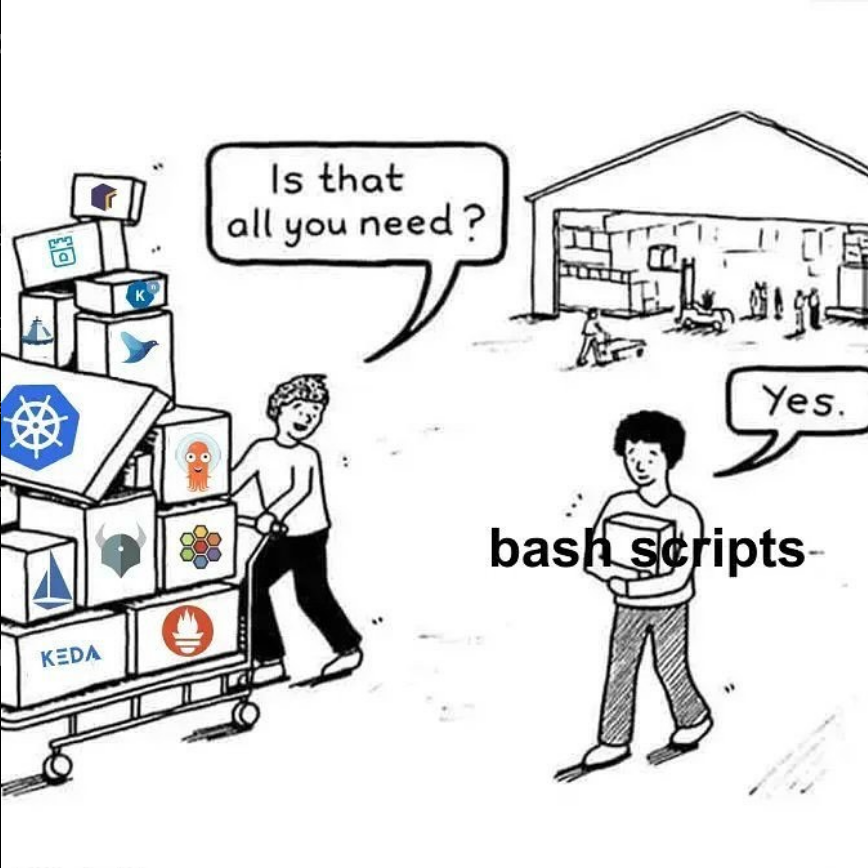
\includegraphics[width=0.4\linewidth] {bashgod}
        \label{fig:bashgod}
    \end{figure}

\end{frame}

% 11 SLIDE
\begin{frame}
    \frametitle{Our first automatization}
    \small We will start with a simple script that will clean up the trash
    \newline then we will backup configs and move on to create hot reloading
    on a generic project.
\end{frame}

\begin{frame}
    \frametitle{Let's talk debugging}
    \footnotesize
    The Bash shell contains no debugger, nor even any debugging-specific commands or constructs
    \begin{figure}

        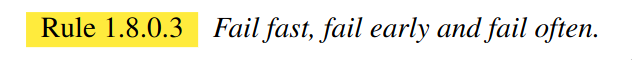
\includegraphics[width=0.6\linewidth, left]{fail}

        \label{fig:fail}

    \end{figure}
    We have some tools to help us with that in shell scripting:
    \begin{itemize}
        \item set -x / -e / -u / -o pipefail
        \item out beloved printf
        \item dtrace
        \item strace
    \end{itemize}
\end{frame}

\begin{frame}
\frametitle{Now cron jobs comes into play}
\small
    One of the most useful tools for automation is cron. \newline
    It allows you to schedule tasks to run at specific times or intervals. \newline
    But there is more! \newline
    \large > anacron
\end{frame}

\begin{frame}
    \frametitle{How does cron/anacron work?}
    \small
    Cron is started from /etc/rc.d/init.d or /etc/init.d when classical sysvinit scripts are used. In case systemd is enabled, then unit file is installed into /lib/sys‐
       temd/system/crond.service and daemon is started by systemctl start crond.service command. It returns immediately, thus, there is no need to need to start it with  the
       \& parameter.
\end{frame}

% 10 SLIDE
\begin{frame}
\frametitle{But there is more! Event driven automation}
\small
    What if we could automate tasks based on events that happen on the system? \newline
    \pause
    In this context, we can take advantage of the Linux kernel's ability to
    notify userspace programs of events that happen on the system. \newline
\end{frame}

% 11 SLIDE
\begin{frame}
\frametitle{What are the events in Linux that we can use?}
    \small
    \begin{block}{Remark}
        We will modify the behavior of the system based on the events throughout
        custom scripts, whose path may differ from one distro to another.
    \end{block}
    \begin{itemize}
        \item openrc/systemd daemons events (init system)
        \item inotify (file system events)
        \item cgroups (resource management)
        \item acpi (power driven events)
        \item udev (device management)
        \item custom hooks and signals
    \end{itemize}
\end{frame}

% 12 SLIDE
\begin{frame}
    \frametitle{Do you really need to compose all the events?}
    \small
    Absolutely not! \newline
    You can use the events that are relevant to your day to day tasks. \newline
\end{frame}
% 13 SLIDE
% 14 SLIDE
% 15 SLIDE
% 16 SLIDE
% 17 SLIDE
\begin{frame}
    \frametitle{Orchestrating multiple servers with Docker}
    \small
    Of course we can use Docker to automate the deployment of our applications
    \begin{figure}
        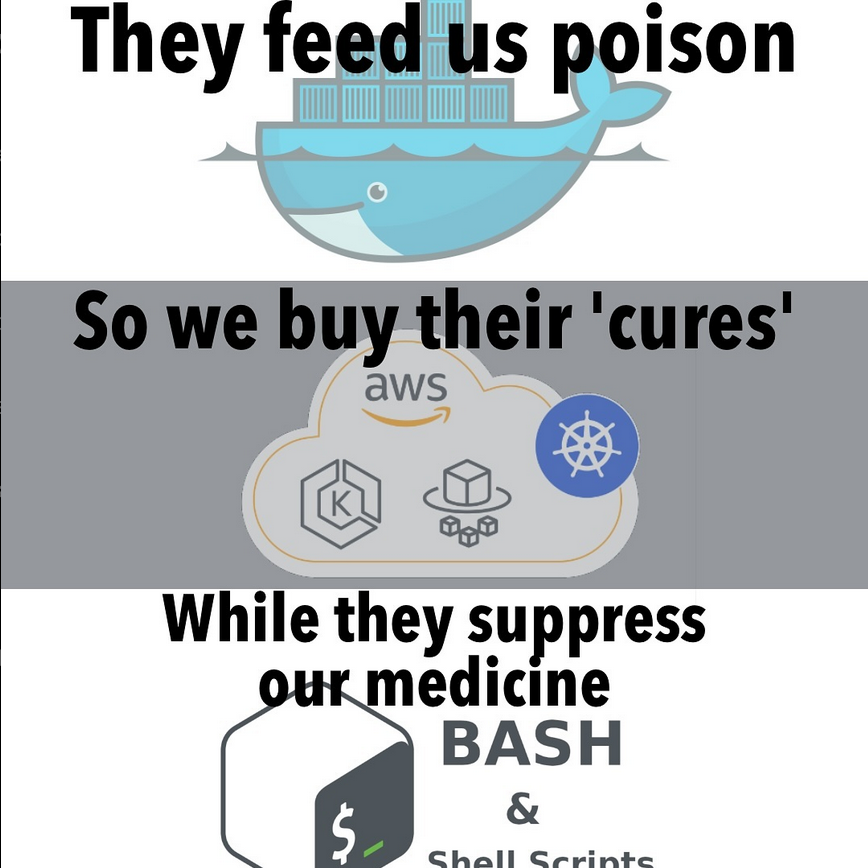
\includegraphics[width=0.4\linewidth] {bash_poison}
        \label{fig:bash_poison}
    \end{figure}
    \footnotesize You can also do this is our beloved shell scripts but I think
    it's convienient to use Docker for this task.
\end{frame}

\begin{frame}
    \frametitle{Install docker}
    \small
    Depending on your distro you can install docker with the package manager
    or you can download the binaries from the official website.
    \newline
    The script:
        curl -fsSL https://get.docker.com -o get-docker.sh
        sudo sh get-docker.sh
    \newline
    also you need to add your user to the docker group
    \newline
    sudo usermod -aG docker \$USER
    \newline
    add the service to the init system
    \newline For openrc: sudo rc-update add docker default
    \newline For systemd: sudo systemctl enable docker
    \newline Now check if docker is running:
    \newline docker - -version
\end{frame}

\begin{frame}
    \frametitle{Manage containers}
\end{frame}
\begin{frame}
    \frametitle{Mock the frontend}
\end{frame}
\begin{frame}
    \frametitle{Mock the backend}
\end{frame}
\begin{frame}
    \frametitle{Mock the database}
\end{frame}

\begin{frame}
    \frametitle{What are we trying to achieve?}
    \small For this example we will try to deploy a simple web application consisting
    of a frontend, backend and a database. \newline
    \newline
    This is very simple but it can be scaled to a more complex situation
    at your work or personal projects.
\end{frame}
% 18 SLIDE
\begin{frame}
    \frametitle{Take it to the final level with Kernel Modules}
    \begin{figure}
        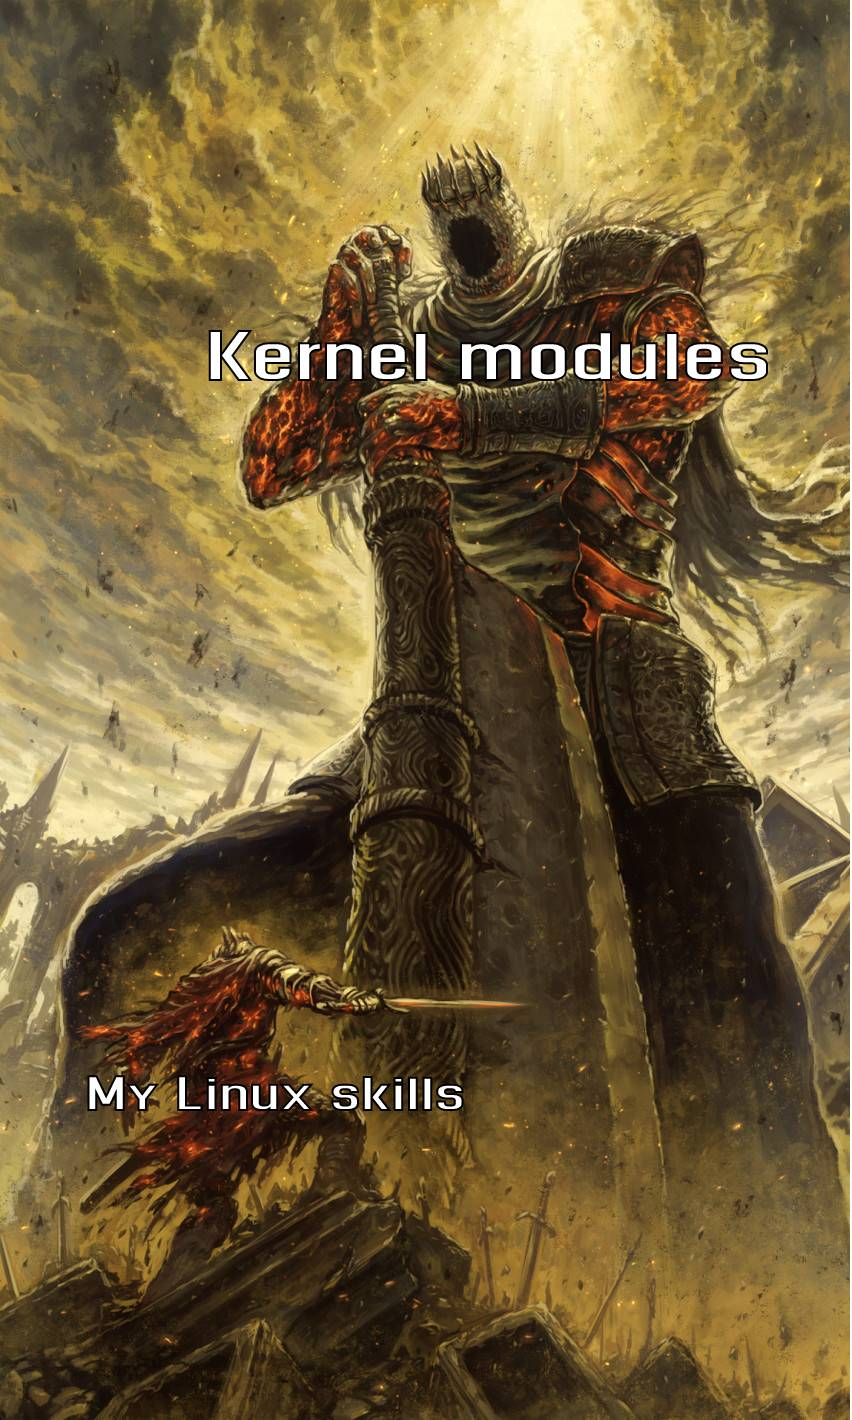
\includegraphics[width=0.35\linewidth] {linuxkernel}
        \label{fig:linuxkernel}
    \end{figure}
    \centering \small{Why do we need kernel modules anyway?}
\end{frame}

\begin{frame}
    \frametitle{Writing your own kernel module}
    \begin{alertblock}{Be aware of the risks}
        \small
        Writing a kernel module is a risky business, as it can crash the system
        if not done properly. \newline
        \newline
        \textbf{But} it can also be a very rewarding experience, as you will
        learn a lot about the kernel and the way it interacts with the hardware.
    \end{alertblock}
    \small
    The risks consists in the fact that you can write to the wrong memory
    address, you can cause a kernel panic, you can cause a deadlock, you can
    cause a memory leak, you can cause a buffer overflow etc.
    \newline
    Also you need to \textbf{pay attention to the future kernel releaseas} as
    the API may change and so your module should do.

\end{frame}

\begin{frame}
    \frametitle{Here we don't have int main() function...}
    \small
    Get rid of the main function, printf, scanf and other functions that are
    not available in the kernel space. \newline \newline
    A kernel module is a piece of code that can be loaded or unloaded
    from the kernel on demand. Hence there will be 2 functions that will
    handle this process: \newline
\end{frame}

\begin{frame}
    \frametitle{Load, unload, debug, repeat}
    \footnotesize
    A basic kernel module consists of the main file and the Makefile.
    \begin{figure}
        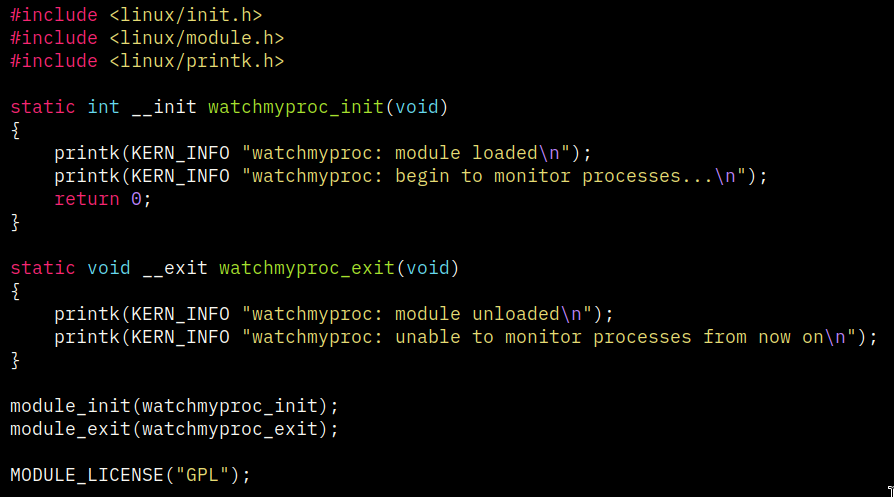
\includegraphics[width=0.7\linewidth] {simplekernel}
        \label{fig:simplekernel}
    \end{figure}
    Now you can compile it with:
    \textbf{make}
    \newline
    and load it with:
    \textbf{sudo insmod watchmyproc.ko}
    \newline
    check the output with:
    \textbf{sudo dmesg}
    \newline
    now you can remove it with:
    \textbf{sudo rmmod watchmyproc}
    \newline
    check the output again to see the module being removed.

\end{frame}

\begin{frame}
    \frametitle{Let the fun begin}
    \small
    We will utilize the kernel module to monitor the processes that are
    running on the system and take some actions based on the events that
    we will receive.
    \newline
    \newline
    We will take advantage of the kernel's ability to notify userspace
    throughout its API.
    \newline
    \newline
    Until now we have used programs that have exposed the kernel API to us
    \textbf{but} now we will use them directly with all the functions
    that are available to us.
\end{frame}

% 19 SLIDE
% \begin{frame}
%     \frametitle{Sample frame title}
%
%     In this slide, some important text will be
%     \alert{highlighted} because it's important.
%     Please, don't abuse it.
%
%     \begin{block}{Remark}
%         Sample text
%     \end{block}
%
%     \begin{alertblock}{Important theorem}
%         Sample text in red box
%     \end{alertblock}
%
%     \begin{examples}
%         Sample text in green box. The title of the block is ``Examples".
%     \end{examples}
% \end{frame}

\begin{frame}
    \frametitle{Resources}
    \small
    I have documented everything in a github repository, where you can find it here:
    \begin{figure}

        
\includegraphics[width=0.4\linewidth]{qr-github}

        \label{fig:qr-github}

    \end{figure}
    \centering \small There will be links, examples we've done today and some
    extra resources for the adventurous ones that want to take the Linux
    journey to the next level.

\end{frame}

\begin{frame}
    \frametitle{Your feedback is important}
    \small
    This is my first workshop and I would like to know your opinion about it.
    \begin{figure}

        
\includegraphics[width=0.4\linewidth]{qr-github}

        \label{fig:qr-github}

    \end{figure}
    \centering \small Please scan the QR code and fill in the form.
\end{frame}

\begin{frame}
    \frametitle{Thank you!}
    \small
    I hope you enjoyed this workshop and that you have learned something new.
    \newline
    \newline
    Now we will have some time to answer your questions.
    \newline
    \newline
    So feel free to ask me anything you want to know.
\end{frame}

\end{document}
